% Choose scrartcl (normal document)
\documentclass[
  bibliography=totoc,     % Literatur im Inhaltsverzeichnis
  captions=tableheading,  % Tabellenüberschriften
  titlepage=false, % Titelseite ist nicht Deckblatt
  twocolumn=true,
  parskip= half,
  abstract=true,
  DIV=25
]{scrartcl}

% Set language here
\usepackage[english]{babel}

\usepackage{fontspec}
\usepackage{amsmath}
\usepackage{amssymb}
\usepackage{mathtools}

%Physics styles
\usepackage[
  math-style=ISO,
  bold-style=ISO,
  sans-style=italic,
  nabla=upright,
  partial=upright
]{unicode-math}

% numbers and units
\usepackage[
  %   locale=DE,
  separate-uncertainty=true,  % use \pm
  per-mode=symbol-or-fraction,
  binary-units=true,
  %per-mode=reciprocal,
  %output-decimal-marker=.,
]{siunitx}

% Fix missing micro sign with TL2017
\sisetup{
  math-micro=\text{μ},
  text-micro=μ,
  range-phrase = -,
  list-separator       = {, },
  list-final-separator = { und },
  range-units = single
}

% Positioning
\usepackage{float}
% Floats inside of section 
\usepackage[section, below]{placeins}
% same for Subsections 
\makeatletter
\AtBeginDocument{%
  \expandafter\renewcommand\expandafter\subsection\expandafter{%
    \expandafter\@fb@secFB\subsection
  }%
}
\makeatother
\floatplacement{figure}{htbp}
\floatplacement{table}{htbp}

% making caption look nice
\usepackage[
  format=plain,
  labelfont=bf,
  font=small,
  width=\linewidth,
]{caption}
\usepackage{subcaption}

% pictures
\usepackage{graphicx}

% Use _ in paths
\usepackage{grffile}

% tables
\usepackage{booktabs}

% optimizing look
\usepackage{microtype}
\usepackage[shortcuts]{extdash}

\usepackage{tikz}
\usepackage{tikz-feynman}

\setmainfont{Libertinus Serif}
\setsansfont{Libertinus Sans}
\setmonofont{Libertinus Mono}
\setmathfont{Libertinus Math}
\DeclareMathAlphabet{\mathcal}{OMS}{cmsy}{m}{n}
\recalctypearea

\usepackage[
  backend=biber,   % use modern biber backend
  autolang=hyphen, % load hyphenation rules for if language of bibentry is not
  % german, has to be loaded with \setotherlanguages
  % in the references.bib use langid={en} for english sources
  urldate=iso,%
  date=iso,%
  style=phys,%
  articletitle=true,biblabel=brackets,%
  chaptertitle=false,pageranges=false,%
  maxnames=2%
]{biblatex}

\usepackage{todonotes}
\presetkeys{todonotes}{inline}{}
%\setuptodonotes{color=lhcb3,size=\tiny}
\usepackage{xfrac}

\usetikzlibrary{patterns}
\usetikzlibrary{angles}
\usepackage{tabularx}

% quotation marks
\usepackage{csquotes}
\usepackage{slashed}
\usepackage{expl3}
\usepackage{xparse}
\usepackage{xcolor}
\usepackage{ifthen}
\usepackage{mleftright}
\usepackage{ragged2e}
% my makros
% useful makros
\ExplSyntaxOn

\DeclareSIUnit\century{century}
\DeclareSIUnit\year{yr}

\makeatletter % allows me to use @
\NewDocumentCommand \showfont {} 
{encoding: \f@encoding{},
  family: \f@family{},
  series: \f@series{},
  shape: \f@shape{},
  size: \f@size{}
}
\NewDocumentCommand \symbfiftextbf {m}
{
    \ifthenelse{\equal{\f@series}{bx}\or\equal{\f@series}{b}}{\symbf{#1}}{#1}
}

\makeatother

\AtBeginDocument{
\let\ltext=\l
\RenewDocumentCommand \l {}
{
    \TextOrMath{ \ltext }{ \mleft }
}
\let\raccent=\r
\RenewDocumentCommand \r {}
{
    \TextOrMath{ \raccent }{ \mright }
}
}
\NewDocumentCommand \dif {}
{
    \mathinner{\symup{d}\mathchoice{\!}{\!}{}{} }
}

\ExplSyntaxOff
\NewDocumentCommand \tindex {mm}
{
    {#1_{\symup{#2}}}
}
\ExplSyntaxOn

\setlength{\delimitershortfall}{-1sp}
\DeclarePairedDelimiter{\abs}{\lvert}{\rvert}
\DeclarePairedDelimiter{\norm}{\lVert}{\rVert}
\DeclarePairedDelimiter\bra{\langle}{\rvert}
\DeclarePairedDelimiter\ket{\lvert}{\rangle}
\DeclarePairedDelimiterX\braket[2]{\langle}{\rangle}{#1 \delimsize\vert #2}

\NewDocumentCommand\xDeclarePairedDelimeter{mmm}
{%
\NewDocumentCommand#1{som}{%
\IfNoValueTF{##2}
    {\IfBooleanTF{##1}{#2##3#3}{\mleft#2##3\mright#3}}
{\mathopen{##2#2}##3\mathclose{##2#3}}%
}%
}
\xDeclarePairedDelimeter{\set}{\lbrace}{\rbrace}

\let\mysubsection=\subsection
\RenewDocumentCommand\subsection{m}
{
    \FloatBarrier
    \mysubsection{#1}
}

\NewDocumentCommand{\anti} {m}
{
    \overline{#1}
}

\AtBeginDocument{
    \RenewDocumentCommand \Re {} {\operatorname{Re}}
    \RenewDocumentCommand \Im {} {\operatorname{Im}}
}

\NewDocumentCommand{\mat}{m}{
    \symbf{#1}
}

\ExplSyntaxOff


% to use the LHCb colors, the same as in the plots
\definecolor{lhcb1}{HTML}{1f77b4}
\definecolor{lhcb2}{HTML}{ff7f0e}
\definecolor{lhcb3}{HTML}{2ca02c}
\definecolor{lhcb4}{HTML}{d62728}
\definecolor{lhcb5}{HTML}{9467bd}
\definecolor{lhcb6}{HTML}{8c564b}
\definecolor{lhcb7}{HTML}{e377c2}
\definecolor{lhcb8}{HTML}{7f7f7f}
\definecolor{lhcb9}{HTML}{bcbd22}
\definecolor{lhcb10}{HTML}{17becf}

\definecolor{mDarkBrown}{HTML}{604c38}
\definecolor{mDarkTeal}{HTML}{23373b}
\definecolor{mLightBrown}{HTML}{EB811B}
\definecolor{mLightGreen}{HTML}{14B03D}
\definecolor{vertexDarkGrey}{HTML}{23373b}
\definecolor{vertexLightGrey}{rgb}{0.833333333,0.8117647064,0.790196078}
\colorlet{vertexDarkRed}{red!70!black}
\colorlet{vertexLightRed}{vertexDarkRed!60!white}
\colorlet{vertexDarkGreen}{green!70!black}
\colorlet{vertexLightGreen}{vertexDarkGreen!50!white}
\colorlet{vertexDarkBlue}{blue!70!black}
\colorlet{vertexLightBlue}{vertexDarkBlue!50!white}


% Hyperlinks
\usepackage[
  allbordercolors = vertexDarkGreen,
  unicode,        % Unicode in PDF-Attributen erlauben
  pdfusetitle,    % Titel, Autoren und Datum als PDF-Attribute
  pdfcreator={},  % ┐ PDF-Attribute säubern
  pdfproducer={}, % ┘
]{hyperref}
% erweiterte Bookmarks im PDF
\usepackage{bookmark}


\title{Fourier Transform of Images}
\subject{Computational Physics -- 08 }
\author{Ludwig Neste}

\addbibresource{references.bib}


\begin{document}

% For the beamer class:
%\begin{frame}
%	\titlepage
%\end{frame}
%\begin{frame}{Table of contents}
%	\setbeamertemplate{section in toc}[sections numbered]
%	\tableofcontents[hideallsubsections]
%\end{frame}

\maketitle

\section{Discrete Fourier Transform}

The \emph{Discrete Fourier Transform (DFT)} of a series of complex numbers $\vec x = x_0, \dots, x_{N-1}$
are the $N$ numbers defined as
\begin{equation}
    X_k = \symcal{F}\left(\vec x\right)_k = \frac{1}{\sqrt{N}}\sum_{n=0}^{N-1} x_n e^{-i\frac{2\pi}{N}n k}.
\end{equation}
For intuitive understanding one can think of $X_k$ as the intensity of the frequency,
$\nu =\frac{\omega}{2\pi}= k / N$ in the signal.

\begin{table}
    \centering
    \caption{Example of the DFT of the sequence 4, 8, 15, 16, 23, 42.}
    \begin{tabular}{S[table-format=1.0] S[table-format=2.0] S[table-format=2.1] >{\hspace{-1em}}c<{\hspace{-.8em}} S[table-format=2.1]}
        \toprule
        {$k$} & {$x_k$} & \multicolumn{3}{c}{$X_k$}               \\
        \midrule
        0     & 4       & 44.1                      & $+i$ & 0.0  \\
        1     & 8       & -2.4                      & $+i$ & 14.8 \\
        2     & 15      & -9.8                      & $+i$ & 9.1  \\
        3     & 16      & -9.8                      & $+i$ & 0.0  \\
        4     & 23      & -9.8                      & $-i$ & 9.1  \\
        5     & 42      & -2.4                      & $-i$ & 14.8 \\
        \bottomrule
    \end{tabular}
\end{table}

For a deeper understanding let's take a step back and remember that Fourier
found that a periodic function can be represented as a weighted sum of cosine and
sine functions.
This does not only apply for continuous, but also discontinuous functions,
such as a square wave.
To put it in a more mathematical way: The
$L^2([0, T])$-space\footnote{This means every complex-valued function defined on $[0, T]$, which's absolute square is integrable over $[0, T]$.}
has the orthonormal basis functions
\begin{equation}
    \phi_k(x)=\exp\left({-2ikx\frac{2\pi}{T}}\right) \quad k\in \mathbb{Z},
\end{equation}
so any function $f(x)\in L^{2}([0, T])$ can be written as
\begin{equation}
    f(x) \equiv \sum_{k=-\infty}^{\infty} \underbrace{\left< f, \phi_k \right>}_{a_k} \phi_k(x)
    = \sum_{k=-\infty}^{\infty} {a_k} \exp\left({-2ikx\frac{2\pi}{T}}\right)
\end{equation}
where $\equiv$ means "equals almost everywhere under the norm induced by the scalar product $\left<\cdot,\cdot\right>$".
This sum is called a Fourier series.
The scalar product (and thus the norm) in this space is
\begin{equation}
    \left< f, g\right> = \int_0^T f(x)g^*(x) \dif x.
\end{equation}
Thus, the Fourier coefficients $a_k$ are
\begin{equation}
    a_k = \int_0^T f(x) \exp\left({ikx\frac{2\pi}{T}}\right) \dif x
\end{equation}
This is a very abstract definition, but if we get used to the math,
this only precises the findings of Fourier: A periodic function
(our functions are restricted to $[0, T]$, but they can be thought of as being periodically continued everywhere else)
can be represented as a weighted (infinite) sum of sines and cosines (in our formulation hidden with the Euler identity in $e^{ix}$).

If we now have a function which is neither confined nor periodic, we can handwavely argue, that $T$ goes to infinity and
that we need a continues set of basis functions. This is a way of approaching the continuous \emph{Fourier Transform (FT)}.
The idea of the FT is to transform the original function $f$ to another function $\hat f$ without loosing any information and thus being
able to transform the function back.
The transformation is similar to the definition of the Fourier coefficients
\begin{equation}
    \hat f(\nu) = \int_{-\infty}^{\infty} f(x) e^{-i2\pi\nu x} \dif x.
\end{equation}
The inverse Fourier transform is given by
\begin{equation}
    f(x) = \int_{-\infty}^{\infty} \hat f(\nu) e^{i2\pi\nu x} \dif \nu.
\end{equation}
For this the function $f: \mathbb{R}\to \mathbb{C}$ only has to be absolutely integrable, so that
$\int_{\mathbb{R}} \abs{f(x)} \dif x$ is defined.

The correctness of the inverse-rule can be shown if we express the Dirac $\delta$-function as
\begin{equation}
    \delta(x) = \int_{-\infty}^{\infty} e^{-i2\pi \nu x} \dif \nu.
\end{equation}

Again $\hat f(\nu)$ can be thought of as the intensity of the frequency $\nu$ in the function. That's
why we name the domain $\nu$ and $\hat f$ is often called $f$ in frequency-space.
This definition is easily extended to functions which take multi-dimensional input $f: \mathbb{R}^n \to \mathbb{C}$
\begin{equation}
    \hat f(\vec \nu) = \int_{\mathbb{R}^n} f(\vec x) e^{-i2\pi\vec \nu \cdot \vec x} \dif{}^n x.
\end{equation}
And the inverse transform likewise.

Now we can motivate the DFT: If we define a function (to be exact: a distribution) as
\begin{equation}
    f(x) = \frac{1}{\sqrt N} \sum_{n=0}^{N-1} x_n\ \delta\left(x-{n}\right)
\end{equation}
the DFT of the points is the FT of this function at the frequencies $k/N$
\begin{equation}
    \begin{split}
        \hat f\left(\frac{k}{N}\right) = \int_{-\infty}^{\infty}  \frac{1}{\sqrt N} \sum_{n=0}^{N-1}
        x_n\ \delta\left(x-{n}\right) e^{-i2\pi\frac{k}{N} x} \dif x\\
        = \frac{1}{\sqrt N} \sum_{n=0}^{N-1} x_n e^{-i2\pi k \frac{n}{N}}
        = X_k.
    \end{split}
\end{equation}
And likewise, if we define the function
\begin{equation}
    F(\nu) = \frac{1}{\sqrt N} \sum_{n=0}^{N-1} X_n\ \delta\left(\nu-{n}\right)
\end{equation}
it's inverse FT at $k/N$ is the inverse DFT of the points $X_k$
\begin{equation}
    \begin{split}
        \hat F\left(\frac{k}{N}\right)
        = \int_{-\infty}^{\infty}  \frac{1}{\sqrt N} \sum_{n=0}^{N-1}
        X_n\ \delta\left(\nu-{n}\right) e^{i2\pi\frac{k}{N} \nu} \dif \nu\\
        = \frac{1}{\sqrt N} \sum_{n=0}^{N-1} X_n e^{i2\pi k \frac{n}{N}}
        = \frac{1}{N} \sum_{n,m=0}^{N-1}
        x_m e^{-i2\pi \frac{n}{N}(m-k)}\\
        =  \sum_{m=0}^{N-1}
        x_m\delta_{m,k} = x_k.
    \end{split}
\end{equation}
Where we have used the relation with the geometric series
\begin{equation}
    \frac{1}{N}
    \sum_{n=0}^{N-1}
    e^{-i2\pi \frac{n}{N}(m-k)}=
    \begin{cases}
        \frac{1-e^{-i2\pi (m-k)}}{1-e^{-i2\pi\frac{m-k}{N}}} = 0 & \forall m\neq k \\
        1                                                        & \forall m=k
    \end{cases}
    = \delta_{m,k}.
\end{equation}
The definition of the function might seem abstract at first glance, but it is nothing
more than a more mathematical way of expressing, that we only have $N$ samples of
an unknown functions at these points.
The normalization factor of $1/\sqrt N$ is chosen so the inverse transform does not rescale
the points.

As with the FT, the DFT is easily enlarged to more dimensions
\begin{equation}
    X_{l,m} = \frac{1}{\sqrt{N_1N_2}}\sum_{j=0}^{N_1-1}\sum_{l=0}^{N_2-1}x_{j,l} \ e^{-i{2\pi}\ \left(\!\frac{lj}{N_1}+\frac{ml}{N_2}\right)}.
\end{equation}
and the inverse
\begin{equation}
    x_{l,m} = \frac{1}{\sqrt{N_1N_2}}\sum_{j=0}^{N_1-1}\sum_{l=0}^{N_2-1} X_{j,l} \ e^{i{2\pi}\ \left(\!\frac{lj}{N_1}+\frac{ml}{N_2}\right)}.
\end{equation}
I chose the three-dimensional example here, since we are going to look at images with a color channel, which is three dimensional data.
Other dimensionalities are analogous.

\subsection{Real Numbered Input Data}
An image will only contain real numbered input values. This yields the following symmetry in the transformation
\begin{equation}
    X_{l,m,n} = X^*_{N_1-l,N_2-m,N_3-m}.
    \label{eqn:realFSymmetry}
\end{equation}
On the one hand, this is a very useful result: If we transform an image consisting of $N$ real numbers,
we do not want to end up with $N$ complex (or equivalently $2N$ real) numbers.
On the other hand this poses a challenge in displaying the transformed image.
Usually we can only display the magnitude of the transformed image.

Since it seems quite artificial to introduce complex numbers in a problem only consisting of real numbers,
for image compression usually a very closely related transform is used, the \emph{Discrete Cosine Transfrom (DCT)}.
It transforms $N$ real-valued input numbers to $N$ real-valued output numbers.
The transform is given by
\begin{equation}
    \begin{split}
        X_k = \symcal{C}\left(\vec x\right)_k = \frac{2c_k}{\sqrt N}\sum_{n=0}^{N-1}x_n \cos \left(\frac{\pi\left(2n+1\right)k}{2N} \right)
        \\
        \text{where }
        c_k =
        \begin{cases}
            \frac{1}{\sqrt{2}} \quad & k=0           \\
            1                        & \text{ else }
        \end{cases}
    \end{split}
\end{equation}
and it's inverse by
\begin{equation}
    x_k = \symcal{C}^{-1}\left(\vec X\right)_k
    =\frac{1}{\sqrt N}\sum_{n=1}^{N-1}c_n X_n \cos \left(\frac{\pi(2k+1)}{2N}n\right).
\end{equation}
\cite{DCT}
The DCT can be calculated using the DFT. An efficient algorithm for this from \cite{DCTUFFT} first reorders the points to
\begin{equation}
    \begin{rcases}
        x'_k       & = x_{2k}  \\
        x'_{N-1-k} & =x_{2k+1}
    \end{rcases}
    k=0,1, \dots, \frac{N}{2}-1
\end{equation}
to obtain the relation
\begin{equation}
    \symcal{C}\left(\vec x\right)_k = X_k =2 c_k
    \Re e^{i\pi\frac{k}{2N}}\symcal{F}^{-1}\left(\vec x'\right)_k
\end{equation}
and it's inverse
\begin{equation}
    \begin{split}
        \symcal{C}^{-1}\left(\vec X\right)_{2k} =& x_{2k} =
        \Re \symcal{F}^{-1}\left\{c_lX_le^{i\frac{\pi l}{2N}}\right\}_k
        \\
        &x_{2k+1} = x_{2(N-1-k)}.
    \end{split}
\end{equation}
Note, that we only need to calculate half of the Fourier coefficients, if we make use of
Equation \eqref{eqn:realFSymmetry}.

\section{The Numerical Implementation: The Fast Fourier Transform}
Firstly, we notice that the multidimensional discrete Fourier transform is
separable into multiple one dimensional DFT, performed one after another.
Thus, we will concentrate on optimizing the one dimensional DFT:
\begin{equation}
    X_{l,m} = \symcal{F} \left\{\symcal{F}\{(x_i)_j\}_m\right\}_l
\end{equation}

We can see that the direct implementation of the DFT is like a matrix-multiplication
\footnote{In fact, it is possible to interpret the DFT as a curve fitting problem with the design matrix $A_{m,n}=e^{-i2\pi\frac{mn}{N}} / \sqrt{N}$.}.
As that, the computational complexity of the bare DFT implementation scales with $\symcal{O}(N^2)$.
But the concrete form of the transform allows us to get down to $\symcal{O}(N\log N)$.
From this scaling law, we can already guess, that we will use a divide-and-conquer algorithm.
The basic idea is to express the Fourier transform of $N$ points in multiple smaller Fourier transforms, and thus dividing and conquering.
Let's assume $N$ is even and observe that
\begin{equation}
    \begin{split}
        X_k &= \frac{1}{\sqrt{N}}\sum_{n=0}^{N-1} x_n e^{-i\frac{2\pi}{N}n k}\\
        &=\frac{1}{\sqrt N}
        \sum_{n=0}^{N/2-1} x_{2n} e^{-i\frac{2\pi}{N}2n k}+
        \frac{1}{\sqrt N}
        \sum_{n=0}^{N/2-1} x_{2n+1} e^{-i\frac{2\pi}{N}(2n+1) k}\\
        &= \frac{1}{\sqrt 2}
        \symcal{F}\left\{x_{2n}\right\}_k
        +\frac{1}{\sqrt 2}
        e^{-i\frac{2\pi}{N}k}\symcal{F}\left\{x_{2n+1}\right\}_k.
    \end{split}
\end{equation}
The last expression is only defined up to $k=N/2$, but for the other half we get
\begin{equation}
    X_{k+\frac{N}{2}}=\frac{1}{\sqrt 2}
    \symcal{F}\left\{x_{2n}\right\}_k
    -\frac{1}{\sqrt 2}
    e^{-i\frac{2\pi}{N}k}\symcal{F}\left\{x_{2n+1}\right\}_k.
\end{equation}
Here we have expressed the DFT of $N$ points as the DFT of the $N/2$ even points and $N/2$ odd points.
This is called the \emph{Fast Fourier Transform (FFT)}, to be precise the radix-2-decimation-in-time Cooley-Tukey algorithm.
It was originally discovered by Gauss, but due to the lack of computers at his time, it was not a very known result.
Cooley and Tukey rediscovered the algorithm 160 years later in the sixties and popularized it.

We can similarly express the inverse DFT by noticing
\begin{equation}
    \symcal{F}^{-1}\left\{x_n\right\}
    =\symcal{F}\left\{x_{N-n}\right\}
    =\symcal{F}\left\{x_{n}^*\right\}^*.
\end{equation}
Thus, we only need the implementation of the DFT to also get the inverse DFT.

The complete divide and conquer in this form only works for $N$, which are powers of two.
But, it is possible to generalize this to any composite number of the form $N=N_1N_2$.
In that case we will combine $N_1$ smaller DFT with a DFT of size $N_2$\footnote{Note that the combination rule for the even $N$ case can be understood as a DFT of two points.}.
For a full description see \cite{CTAlg}.
Note that this yields problems, if our input data has prime-number length, for this special case there
exist an algorithm allowing the DFT of prime-number-sized points in $N\log N$ time, using group-theory
of prime-numbered modulo groups. The algorithm is called \emph{Rader's algorithm}, see \href{https://en.wikipedia.org/wiki/Rader%27s_FFT_algorithm}{en.wikipedia.org/wiki/Rader\%27s\_FFT\_algorithm}.

\subsection{Code}
The code which produced the results is written in \texttt{C++}.
No numerical algorithms outside the standard template library were used, which
means I implemented a version of the FFT and DCT myself.
The code makes full use of every prime factor of $2$ in the number of transformed points,
but not the full powered Tukey-Cooley algorithm, since an efficient implementation of that
requires complicated reordering of the input numbers.
The used algorithm can handle arbitrary length input data, which makes it
more general than most implementations found online, since they are usually only implemented
for powers of 2.
Nonetheless, the implementation should be viewed more as a toy-implementation for testing
and can't compete with industry-grade optimized algorithms.
The FFT, DCT and their respective inverses where implemented in a generic fashion,
so that they can be used on any datastructure supporting the square-bracket indexing
operator. Thus, it can be used on raw pointers as well as on higher level structures
like vectors.

The images in the Fourier space were represented by complex matrices from the \texttt{Eigen}
library.
To handle images, as well as image-input and -output the Boost Generic Image Library \texttt{Boost::GIL} was used.

\section{Applications}
One of the most notable places the Fourier transform appears in physics is the
Fraunhofer-diffraction equation. In the far-field approximation, the diffraction image
of an incoming planar wave is proportional to the 2D-Fourier transform of the aperture:
\begin{equation}
    A(x, y, z) \propto \iint_{\symup{Aperture}}\hspace{-3em} e^{-i\frac{2\pi}{\lambda z}(x'x+y'y)} \dif x' \dif y'
\end{equation}
Thus, if we use a DFT of an image resembling an aperture, we can numerically approximate the diffraction image.
Every photograph taken is slightly distorted through diffraction effects through the aperture.
In space-telescopes for example the reflection mirror needs to be attached to the rest of the satellite,
and the light from stars is diffracted at the attached rods, which creates the typical 4 or 6-fold diffraction
symmetry of star-pictures.
This can be removed from images through image editing in Fourier-space.

Another application is the lossy compression of images, sound and other media types.
An image can be for example saved by performing a DCT, reducing the amount
of different points by quantizing in the frequency space.
This is what (among other tricks) the \texttt{.jpg} image format does.

Images can also be enhanced with Fourier transform. Assume for example we take a photograph through an insect-net.
We will have periodic information overlaying the picture. This can be easily removed in Fourier space.
Generally, a lot of interesting edits can be performed in Fourier space, having complex outcome in real space.
And by removing high-frequencies the sharpness can be increased and by doing the inverse the image will be blurred.



\section{Results}
All the implemented transforms where tested for correctness by comparing the output
of my implementation to other reference-implementations, like matlab's or scipy's.
The implementation was also tested for speed depending on the length of the input.
For a given input length the FFT algorithm was performed multiple times with random numbers
and the
runtime was measured and averaged. The number of times the algorithm was evaluated
was chosen, such that the uncertainty of the average was below \SI{10}{\nano\second}.
While the actual numbers will be more or less uninteresting, it is possible to see
the $\symcal{O}(N\log N)$ scaling for powers of 2, as shown in \autoref{fig:timesp2}.
Especially for higher-length input the scaling is fulfilled, but for short length
input there is too much overhead, and thus the numbers are not following $N\log N$ perfectly there.

\begin{figure}[htbp]
    \centering
    \includegraphics[width=\linewidth]{build/plots/times_p2.pdf}
    \caption{Runtime of the toy FFT algorithm in double-logarithmic-scaling depending on the length of the input sequence.
        Each random-number input was transformed multiple time and the results were averaged.
        The function $t(N)=c\times N\log N$ is fitted to the measurements, as we expect this scaling for
        input lengths in the form of $2^p$. }
    \label{fig:timesp2}
\end{figure}

For arbitrary sized input, the actual runtime of this algorithm depends heavily on
the number of two's in the prime-factor decomposition of the input-length.
In easier words: the FFT of 48 numbers should be roughly twice as fast as 56, even though
56 is the higher number.
The reason is 48 is divisible by 2 4 times ($48=2^4\cdot 3$), where 56 is only divisble by
2 3 times ($56=2^3\cdot 7$).
This is also clearly seen in the data, as \autoref{fig:times} shows.
\begin{figure}[htbp]
    \centering
    \includegraphics[width=.5\textwidth]{build/plots/times_lin_c.pdf}
    \caption{Averaged runtime of the implemented toy FFT algorithm on random numbers depending on the input length.
        A clear separation of the runtime scaling is seen. The data-points are colored
        depending on the number of times the input length is divisible by 2.}
    \label{fig:times}
\end{figure}


\subsection{Depicting the Fourier Space}
A digital image is nothing more than $N=h\cdot w\cdot C$ numbers $x_{k,l,c}$
\footnote{$k=0,\dots, h-1\quad l=0,\dots,w-1\quad c=0,\dots,C-1$}
between $0$ and $1$.
Where $w$ is the width, $h$ is the height and $C$ is the number of channels of the image.
There are a lot of different types of images out there, with different channel numbers and interpretation
of them (different color encodings, transparent images, etc.), but we will focus on the
case of grayscale $c=1$ or colored RGB $C=3$ pictrues.
The interpretation of the number in grayscale images is the illumination of the pixel ranging from $0=$~off~$=$~black
to $1=$~on~$=$~white.
In colored RGB images, we have three channels: Red (R), Green (G), Blue (B). Where we can light up each color seperately.
Because of how the eye works, we are able to trick the brain into perceiving most of the colors by just
mixing these three.
The numbers are usually not stored as floating point numbers, but as unsigned integers, most commonly 8-bit unsigned integers.
This means that 1 is stored as 255 and all the numbers are mapped in an equally spaced fashion.
If we have multiple channels, we will Fourier transform each channel separately
\begin{equation}
    X_{k,l,c} = \frac{1}{\sqrt{hw}}\sum_{n=0}^{h-1}\sum_{m=0}^{w-1}x_{n,m,c} \ e^{-i{2\pi}\ \left(\!\frac{kn}{h}+\frac{lm}{w}\right)}.
\end{equation}
In the Fourier space each pixel is a complex number.
We usually visualize the magnitude and the phase (the argument) of each number.
Because the magnitude of the Fourier transformed numbers is not guaranteed
to be between 0 and 255, we scale the Fourier transformed numbers in such a way,
that the highest is 255 and the lowest is 0
\begin{equation}
    \abs {X'_{k,l,c}} = 255\frac{\abs {X_{k,l,c}}-\min_{n,m} \abs {X_{n,m,c}}}{\max_{n,m} \abs {X_w{n,m,c}}-\min_{n,m} \abs {X_{n,m,c}}}.
\end{equation}
We also scale the phases to the range of $(0, 255)$
\begin{equation}
    \arg {X'_{k,l,c}} = 255\frac{\arg X_{k,l,c}}{2\pi}.
\end{equation}
This mode of visualization can be seen in \autoref{subfig:ftm_n} to \autoref{subfig:ftp_n}.
\begin{figure}[htbp]
    \centering
    \begin{subfigure}[h]{.9\linewidth}
        \centering
        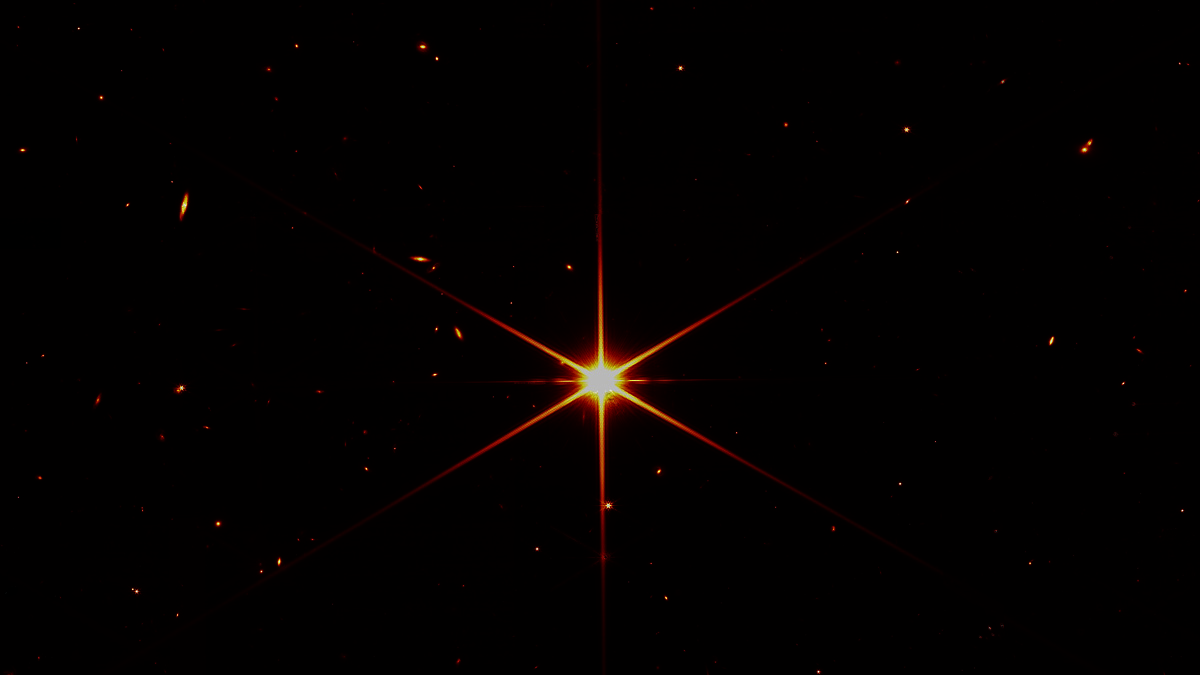
\includegraphics[width=\linewidth]{images/webb.png}
        \caption{Original}
    \end{subfigure}
    \begin{subfigure}[h]{.9\linewidth}
        \centering
        \includegraphics[width=\linewidth]{build/output/webb_mag_n.png}
        \caption{Fourier Transform Magnitude}
        \label{subfig:ftm_n}
    \end{subfigure}
    \begin{subfigure}[h]{.9\linewidth}
        \centering
        \includegraphics[width=\linewidth]{build/output/webb_phase_n.png}
        \caption{Fourier Transform Phase}
        \label{subfig:ftp_n}
    \end{subfigure}
    \begin{subfigure}[h]{.9\linewidth}
        \centering
        \includegraphics[width=\linewidth]{build/output/webb_mag_log.png}
        \caption{Fourier Transform magnitude in logarithmic space}
        \label{subfig:ftm_log}
    \end{subfigure}
    \begin{subfigure}[h]{.9\linewidth}
        \centering
        \includegraphics[width=\linewidth]{build/output/webb_mag.png}
        \caption{FT Magnitude in logarithmic space and rearranged}
        \label{subfig:ftm}
    \end{subfigure}
    \caption{An example of the Fourier transform. The image is the first calibration picture of the new James-Webb space telescope. }
    \label{fig:fourier_example_n}
\end{figure}

As you can see in the example image, the Fourier magnitude is mostly black, and the phases appear to be noise to the eye.
To better distinguish small features, we will now switch to logarithmic color-space for the magnitude
\begin{equation}
    \abs {X''_{k,l,c}} = 255\frac{\log \abs {X_{k,l,c}}-\min_{n,m} \log\abs {X_{n,m,c}} } {\max_{n,m} \log\abs {X_{n,m,c}}-\min_{n,m} \log\abs {X_{n,m,c}}}.
\end{equation}
This is depicted in \autoref{subfig:ftm_log}.
Finally, to better resemble the symmetries in the Fourier space and
to have low frequencies in the middle of the picture, and high frequencies outside,
the indices are shifted
\begin{equation}
    k' = \lfloor k+h/2\rfloor \mod h \qquad l'=\lfloor l+w/2\rfloor\mod w.
\end{equation}
This will be our method of visualization from now on and can be seen in \autoref{subfig:ftm}.

\subsection{Editing in Fourier Space}
If we now modify the numbers in the Fourier space and transform the modified numbers back,
we can achieve complex-looking outcome.
For example, if we take the high frequencies in the image away, we are only left with the
"long-range" information, but the "short-range" information is lost.
This means the image will appear to be blurred.
Taking away the high frequencies can be done in multiple ways.
We can just remove the highest frequencies combining the axes by calculating
$(k'-h/2)^2+(l'-w/2)^2 < r^2$ for some $r$ and setting the pixel in Fourier space to 0, if
this evaluates to false. We can also do this for each axis independently
($(k'-h/2)^2<r_y^2$, $(l'-w/2)^2<r_x^2$).
With these hard cut-offs it is easy to see periodic artifacts in the image.
If we do not want that, we can apply a smooth filter.
A selection of different blurring techniques can be seen
in \autoref{fig:blur_2} to \autoref{fig:blur_smooth}.

\begin{figure}[htbp]
    \centering
    \begin{subfigure}[h]{.49\linewidth}
        \centering
        \includegraphics[width=.9\linewidth]{build/output/dune_mag.png}
        \caption{Fourier space}
    \end{subfigure}
    \begin{subfigure}[h]{.49\linewidth}
        \centering
        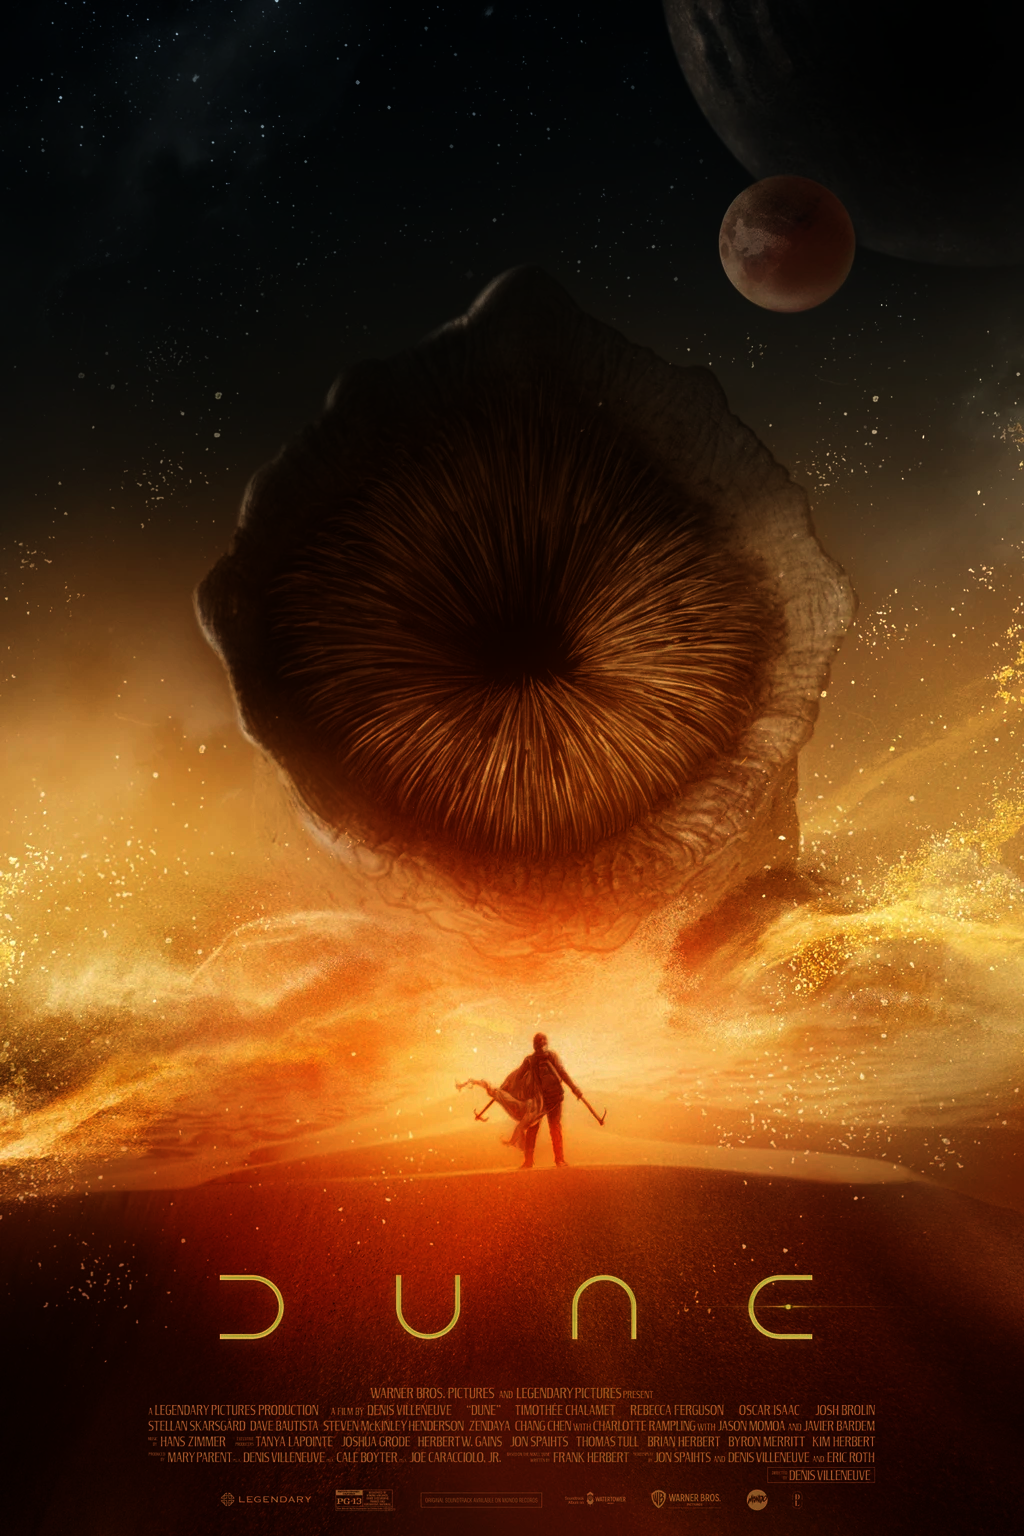
\includegraphics[width=.9\linewidth]{images/dune.png}
        \caption{Original}
    \end{subfigure}\
    \caption{The movie poster of Dune (2021) which serves as an example image being blurred in this section.}
    \label{fig:dune_orig}
\end{figure}

\begin{figure}[htbp]
    \centering
    \begin{subfigure}[h]{.49\linewidth}
        \centering
        \includegraphics[width=.9\linewidth]{build/output/dune_blur2_mask.png}
        \caption{Edit in Fourier space }
    \end{subfigure}
    \begin{subfigure}[h]{.49\linewidth}
        \centering
        \includegraphics[width=.9\linewidth]{build/output/dune_blur2.png}
        \caption{Transformed back to real space}
    \end{subfigure}\
    \caption{The poster above blurred by only keeping the innermost frequencies with a radius of $20\%$ of the width.}
    \label{fig:blur_2}
\end{figure}
\begin{figure}[htbp]
    \centering
    \begin{subfigure}[h]{.49\linewidth}
        \centering
        \includegraphics[width=.9\linewidth]{build/output/dune_blur1_mask.png}
        \caption{Edit in Fourier space }
    \end{subfigure}
    \begin{subfigure}[h]{.49\linewidth}
        \centering
        \includegraphics[width=.9\linewidth]{build/output/dune_blur1.png}
        \caption{Transformed back to real space}
    \end{subfigure}\
    \caption{The poster blurred by only keeping the innermost frequencies with a radius of $10\%$ of the width. This is a circular filter.}
    \label{fig:blur_2}
\end{figure}
\begin{figure}[htbp]
    \centering
    \begin{subfigure}[h]{.49\linewidth}
        \centering
        \includegraphics[width=.9\linewidth]{build/output/dune_rect_mask.png}
        \caption{Edit in Fourier space }
    \end{subfigure}
    \begin{subfigure}[h]{.49\linewidth}
        \centering
        \includegraphics[width=.9\linewidth]{build/output/dune_blur_rect.png}
        \caption{Transformed back to real space}
    \end{subfigure}\
    \caption{The poster blurred by only keeping the $10\%$ innermost frequencies along each axis independently. This is a rectangular filter.}
    \label{fig:blur_rect}
\end{figure}
\begin{figure}[htbp]
    \centering
    \begin{subfigure}[h]{.49\linewidth}
        \centering
        \includegraphics[width=.9\linewidth]{build/output/dune_blur_smooth_mask.png}
        \caption{Edit in Fourier space }
    \end{subfigure}
    \begin{subfigure}[h]{.49\linewidth}
        \centering
        \includegraphics[width=.9\linewidth]{build/output/dune_blur_smooth.png}
        \caption{Transformed back to real space}
    \end{subfigure}\
    \caption{The poster blurred by only multipliying each pixel in the Fourier space with $\exp(-0.001 ((k'-h/2)^2+(l'-w/2)^2))$, where $k', l'$ are the shifted indices from above. This is a Gaussian filter.}
    \label{fig:blur_smooth}
\end{figure}


If we do the opposite and take away some low frequencies, we are sharpening the image.
If we take it to the extreme and remove most low frequencies, we have edge detection.
\begin{figure}[htbp]
    \centering
    \begin{subfigure}[h]{.49\linewidth}
        \centering
        \includegraphics[width=.9\linewidth]{build/output/blackhole_sharp_smooth_mask.png}
        \caption{Fourier space}
    \end{subfigure}
    \begin{subfigure}[h]{.49\linewidth}
        \centering
        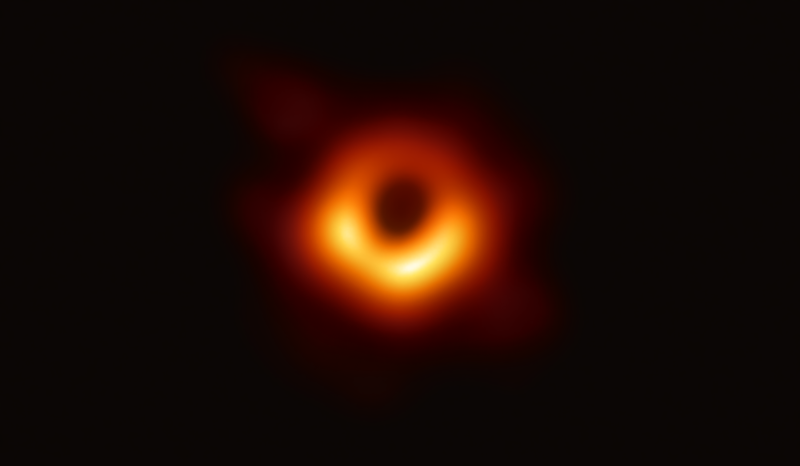
\includegraphics[width=.9\linewidth]{images/blackhole.png}
        \caption{Original}
    \end{subfigure}\
    \caption{The movie poster of Dune (2021) which serves as an example image being blurred in this section.}
    \label{fig:dune_orig}
\end{figure}

\newpage
\printbibliography

\end{document}

